\documentclass
% Uncomment to get one page per frame
%[handout]
{beamer}

\usepackage{amsfonts}
\usepackage{amsmath}
\usepackage{longtable}
\usepackage{csquotes}
\usepackage{standalone}

\usepackage{graphicx}
\graphicspath{{../pictures/}}

\usepackage{tikz}
\usetikzlibrary{shapes, calc, arrows, decorations.markings,
  decorations.pathmorphing, decorations, patterns, chains, snakes,
  backgrounds, positioning, fit, petri}
\newcommand{\inputpicture}[1]{\input{../drawings/#1}}

\newcommand{\reg}{\textsuperscript{\textregistered}}

\usepackage{listings}
\lstset{language=C, basicstyle=\ttfamily, breaklines=true, keepspaces=true,
  keywordstyle=\color{blue}}

\usepackage{bytefield}

\usefonttheme{professionalfonts}
\usefonttheme{serif}
\usepackage{fontspec}
\setromanfont{CMU Serif}
\setsansfont{CMU Sans Serif}
\setmonofont{CMU Typewriter Text}

\newcommand{\No}{{\fontfamily{lmr}\selectfont \textnumero}}

\usepackage{hyperref}
\hypersetup{colorlinks=true, linkcolor=black, filecolor=black, citecolor=black,
  urlcolor=blue , pdfauthor=Evgenii Iuliugin <yulyugin@gmail.com>,
  pdftitle=Fundamentals of Full-Platform Simulation}

\usepackage{underscore}
\usepackage{amsthm}

\subtitle{Fundamentals of Full-Platform Simulation}
\subject{Lecture}
\date{\today}

\author[Evgenii Iuliugin]{
  Evgenii Iuliugin, \small{\href{mailto:yulyugin@gmail.com}{yulyugin@gmail.com}}}
\typeout{Copyright 2021 Evgenii Iuliugin}
\institute{Moscow Institute of Physics and Technology}

\usepackage[bibencoding=inputenc, backend=biber, language=auto,
  style=alphabetic]{biblatex}
\addbibresource{../common/virtualization.bib}
\addbibresource{../common/modelling-languages.bib}
\addbibresource{../common/parallel-simulation.bib}

\usetheme{Madrid}
\setbeamertemplate{navigation symbols}{}

\definecolor{miptdark}{RGB}{25,52,104}
\definecolor{miptlight}{RGB}{1,114,192}
\setbeamercolor{author in head/foot}{fg=white, bg=miptlight}
\setbeamercolor{title in head/foot}{fg=white, bg=miptdark}

\makeatletter
\setbeamertemplate{footline}{%
  \leavevmode%
  \hbox{%
    \begin{beamercolorbox}[wd=.15\paperwidth,ht=2.25ex,dp=1ex,center]{author in head/foot}%
      \usebeamerfont{author in head/foot}\insertshortauthor
    \end{beamercolorbox}%
    \begin{beamercolorbox}[wd=.77\paperwidth,ht=2.25ex,dp=1ex,center]{title in head/foot}%
      \usebeamerfont{title in head/foot}\inserttitle
    \end{beamercolorbox}%
  }%
  \begin{beamercolorbox}[wd=.08\paperwidth,ht=2.25ex,dp=1ex,right]{date in head/foot}%
    \usebeamerfont{date in head/foot}%
    \usebeamertemplate{page number in head/foot}%
    \hspace*{2ex}
  \end{beamercolorbox}
  \vskip-1pt%
}
\makeatother

\newcommand{\startslides}{
  {\setbeamertemplate{footline}{}
  \begin{frame}
      \maketitle
  \end{frame}
  }

  \addtocounter{framenumber}{-1}

  \begin{frame}{\inserttitle}
      \tableofcontents
  \end{frame}
}

\newcommand{\finalslide}{{
  \setbeamertemplate{footline}{}

  \begin{frame}

  {\huge{Thank you!}\par}

  \vfill
  Slides and material are available at
  \url{https://github.com/yulyugin/sim-lectures}
  \vfill

  \tiny{\textit{Note}: All trademarks are the property of their respective
    owners. The presented point of view reflects the personal opinion of
    the author.

    %All the materials are licensed under the Creative Commons
    %Attribution-NonCommercial-ShareAlike 4.0 Worldwide. To view a copy of this
    %license, visit \url{http://creativecommons.org/licenses/by-nc-sa/4.0/}.
  }
  \end{frame}
}\addtocounter{framenumber}{-1}}

\title{Event-Driver Simulation. Multi-processor Simulation}

% TODO: It would be good to explain how hardware works in a bit more detail
% Then map that to events vs continuous processes.
% The word "transaction" is missing. It should be in here.
%
% Would also be good with a diagram explaining the model of execution with
% different devices tied to different processors like it is in Simics, vs
% single global time. That is a fundamental design choice.
%
% Question of truth in the simulator - Simics lets whatever is the result be
% the result vs. quite a few academic approaches that instead try to detect
% causal violations from temporal decoupling and roll back.

\begin{document}

\startslides

\begin{frame}{On the Previous Lectures:}
\begin{itemize}
\item Processor simulation:
  \begin{itemize}
  \item Interpreters (switched, threaded, cached) --- \textbf{slow}.
  \item Binary translators (templates, IR) --- \textbf{faster} but still
    \textbf{slow}
  \item Direct execution (scanning, HW support) --- almost
    \textbf{the fastest}.
  \end{itemize}
\item{<<Gear shifting>> for processor simulation modes.}
\end{itemize}
\end{frame}

\begin{frame}{Questions}
\begin{itemize}
\item When direct execution can be used?\pause
\item Why <<naive>> approach doesn't work?\pause
\item How the problems can be solved?\pause
\item Other areas of application for patching mechanism?
\end{itemize}
\end{frame}

\begin{frame}{Simulated System}
\centering
% TODO: add a link from APIC to addr-decoder.
% Not important for this presenation but the link exists.
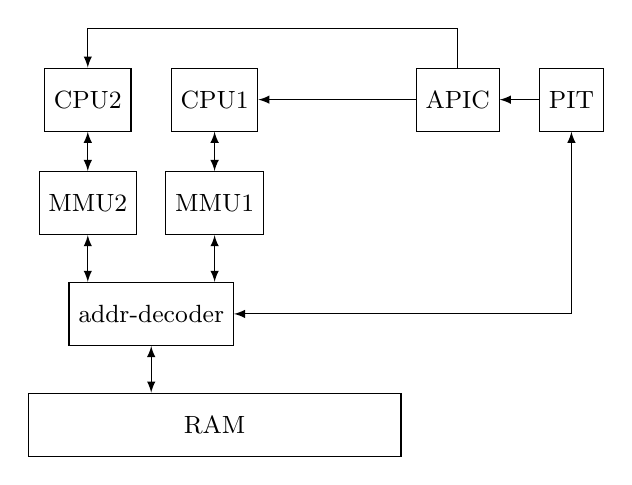
\begin{tikzpicture}[>=latex, font=\small, node distance = 0.5cm]

\begin{scope}[minimum height=0.8cm]
    \node[draw, ] (cpu) {CPU1};
    \node[draw, below=of cpu] (mmu) {MMU1};

    \node[draw, left=of cpu] (cpu2) {CPU2};
    \node[draw, below=of cpu2] (mmu2) {MMU2};
    \node[draw, right=2cm of cpu, ] (pic) {APIC};

    \coordinate[above=of pic] (op);
    \coordinate (mp) at (barycentric cs:mmu=0.5,mmu2=0.5);
    \node[draw, below=1cm of mp] (addr-decoder) {addr-decoder};

    \node[draw, below=2cm of mmu, text width=4.5cm, align = center, ] (dram) {RAM};
    \node[draw, right=of pic, ] (pit) {PIT};
\end{scope}

\draw[<->] (cpu) -- (cpu |- mmu.north);
\draw[<->] (cpu2) -- (cpu2 |- mmu2.north);

\draw[<->] (mmu) -- (mmu |- addr-decoder.north);
\draw[<->] (mmu2) -- (mmu2 |- addr-decoder.north);

\draw[<->] (addr-decoder) -| (pit);
\draw[<->] (addr-decoder) -- (addr-decoder |- dram.north);

\draw[->, ] (pic) -- (cpu);
\draw[->, ] (pit) -- (pic);
\draw[->, ] (pic) -- (op) -| (cpu2);
\end{tikzpicture}
\end{frame}

\section{Timer}

\begin{frame}{Example \No1: Timer}
\centering
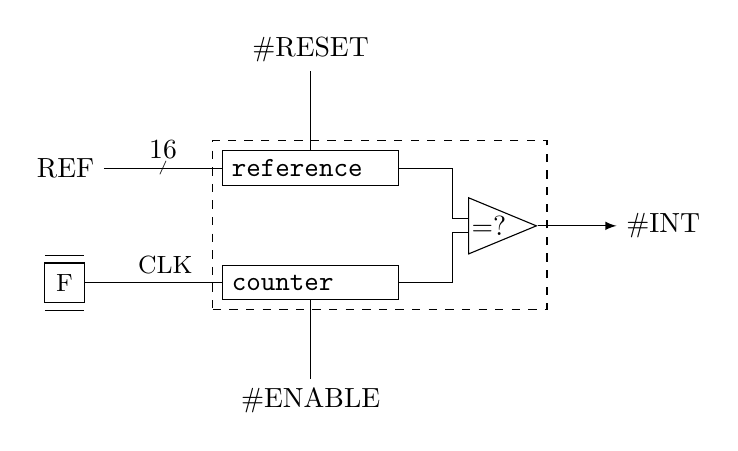
\begin{tikzpicture}[>=latex]
\coordinate (center) at (0,0);
\node[draw, text width = 2cm, above = 0.5 cmof center] (reference) {\texttt{reference}};
\node[draw, text width = 2cm, below = 0.5cm of center] (counter) {\texttt{counter}};
\node[draw, text width = 0.4cm, right = 2cm of center, shape = isosceles triangle, inner sep=1dd] (comparator) {=?};
\node[right = of comparator] (int) {\#INT};
\node[above = of reference] (reset) {\#RESET};
\node[below = of counter] (enable) {\#ENABLE};
\node[left = 1.5cm of reference] (ref-input) {REF};
\node[left = 0.25cm of counter.north west] (clk) {\small{CLK}};

% draw a quartz
\coordinate (quartz) at ([xshift = -2cm]counter.west);
 \node[]  at (quartz) {\small{F}};
\draw (quartz) ++(-0.25,0.25) rectangle ++(0.5,-0.5);
\draw (quartz) ++(-0.25,0.35) -- ++ (0.5,0);
\draw (quartz) ++(-0.25,-0.35) -- ++ (0.5,0);
\draw (reset) -- (reference);
\draw (enable) -- (counter);

% draw wires
\draw (reference.east) -| ([xshift = -0.2cm]comparator.160) -- (comparator.160);
\draw (counter.east) -| ([xshift = -0.2cm]comparator.200) -- (comparator.200);
\draw (ref-input) -- (reference) node[midway] {\tiny{/}} node[midway, above] {16};
\draw (quartz) ++(0.25,0) -- (counter);
\draw[->] (comparator) -- (int);
\node[draw, dashed, fit = (reference) (counter) (comparator)] {};
\end{tikzpicture}
\end{frame}

\begin{frame}{Timing Diagram}
\centering
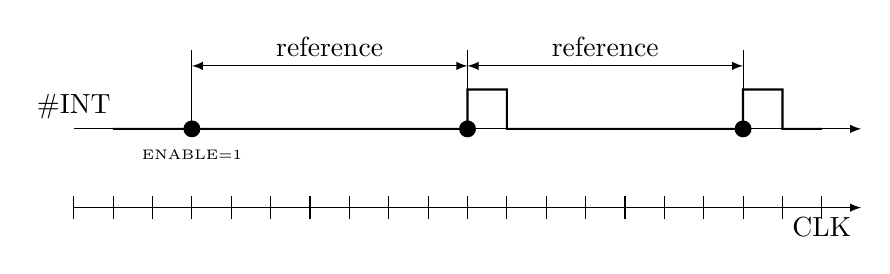
\begin{tikzpicture}[>=latex]
% set clock and #INT time lines
\draw[->] (0,0) -- (10,0) node[pos=0.95, below] {CLK};
\draw[->] (0,1) -- (10,1) node[pos=0.0, above] {\#INT};

\foreach \x in { 0, 1, 2, 3, 4, 5, 6, 7, 8, 9, 10, 11, 12, 13, 14, 15, 16, 17, 18, 19} {
    \draw (\x/2,-0.15) -- (\x/2,0.15)  {};
    \coordinate (tick\x) at (\x/2, 1);
};

\draw[fill=black] (tick3) circle (0.1cm);
\node[below = 0.15cm of tick3] (event-enable) {\tiny{ENABLE=1}};

\draw[fill=black] (tick10) circle (0.1cm);
\draw[fill=black] (tick17) circle (0.1cm);
\draw (tick3)  -- ++(0, 1);
\draw (tick10) -- ++(0, 1);
\draw (tick17) -- ++(0, 1);
\draw[<->] ([yshift=0.8cm]tick3) -- ([yshift=0.8cm]tick10) node[midway, above] {reference};
\draw[<->] ([yshift=0.8cm]tick10) -- ([yshift=0.8cm]tick17) node[midway, above] {reference};

% The actual #CLK plot
\draw[thick] (tick1) -- (tick10) -- ++(0, 0.5) -- ++(0.5, 0) --
            (tick11) -- (tick17) -- ++(0, 0.5) -- ++(0.5, 0) -- (tick18) -- (tick19);

\end{tikzpicture}
\end{frame}

\begin{frame}[fragile]{Simulation With a Fixed Step Size}
\begin{lstlisting}
on_clk() {
  if (enable) counter +=1;
  if (counter == reference) {
      raise_int();
      counter = 0;
  } else {
      lower_int();
  }
}

on_reset() {
    reference = 0;
    counter = 0;
    enable = 0;
}
\end{lstlisting}
\end{frame}

\begin{frame}{Typical Timer Characteristics}
\begin{itemize}
    \item $\mathsf{F} \approx 10$ MHz,
    \item $\mathsf{reference} > 10^3$,
    \item \#RESET --- no more than one per $\approx 100$ seconds.
\end{itemize}
\vfill
$\Rightarrow$ externally visible effect (\#INT) occurs approximately once per
$10^3$ cycles.
\end{frame}

\begin{frame}{Optimization}
No modeling for externally invisible actions.
\vfill
\centering
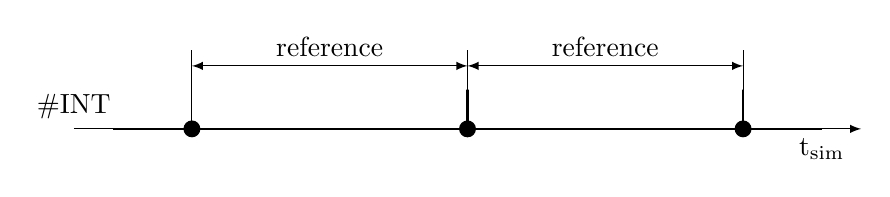
\begin{tikzpicture}[>=latex]
% set clock and #INT time lines
\draw[->] (0,1) -- (10,1) node[pos=0.0, above] {\#INT} node[pos=0.95, below] {t\textsubscript{sim}};

\foreach \x in { 0, 1, 2, 3, 4, 5, 6, 7, 8, 9, 10, 11, 12, 13, 14, 15, 16, 17, 18, 19} {
    \coordinate (tick\x) at (\x/2, 1);
};

\draw[fill=black] (tick3) circle (0.1cm);

\draw[fill=black] (tick10) circle (0.1cm);
\draw[fill=black] (tick17) circle (0.1cm);
\draw (tick3)  -- ++(0, 1);
\draw (tick10) -- ++(0, 1);
\draw (tick17) -- ++(0, 1);
\draw[<->] ([yshift=0.8cm]tick3) -- ([yshift=0.8cm]tick10) node[midway, above] {reference};
\draw[<->] ([yshift=0.8cm]tick10) -- ([yshift=0.8cm]tick17) node[midway, above] {reference};

% The actual #CLK plot
\draw[thick] (tick1) -- (tick10) -- ++(0, 0.5) -- ++(0, -0.5) --
            (tick11) -- (tick17) -- ++(0, 0.5) -- ++(0, -0.5) -- (tick18) -- (tick19);
\end{tikzpicture}
\end{frame}

\begin{frame}[fragile]{Discrete Event Simulation}
\begin{lstlisting}
typedef struct event {
    time_t delta;
    dev_t *device;
    (*function)(dev_t *device);
} event_t;

event_t *event_queue;
time_t sim_time = 0;
for (event_t *e; e != NULL;
     e = next_event(&event_queue)) {
    e->function(e->device);
    sim_time += e->delta;
}
\end{lstlisting}
\end{frame}

\section{Delayed Response}

\begin{frame}{Example \No2: Waiting for a Response}
\begin{center}
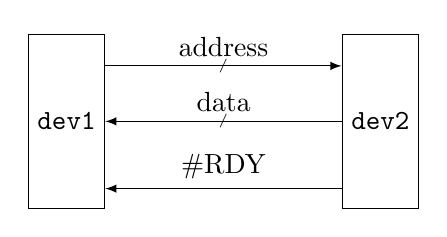
\begin{tikzpicture}[>=latex]
\node[draw, inner ysep=1cm] (dev1) {\texttt{dev1}};
\node[draw, inner ysep=1cm, right= 3cm of dev1] (dev2) {\texttt{dev2}};

\draw[->] (dev1.55) -- (dev2.125) node[midway] {\tiny{/}} node[midway, above] {address};

\draw[->] (dev2) -- (dev1) node[midway] {\tiny{/}} node[midway, above] {data};

\draw[->] (dev2.240) -- (dev1.300) node[midway, above] {\#RDY};
\end{tikzpicture}
\end{center}

\begin{enumerate}
\item Request from \texttt{dev1}: \texttt{address}.
\item \texttt{dev2} calculates \texttt{data}.
\item \texttt{dev2} notifies \texttt{dev1} about data readiness
  \textit{after some time} $\Delta T$ by \#RDY.
\item \texttt{dev1} works independently from \texttt{address} request to \#RDY
  response.
\end{enumerate}
\end{frame}

\begin{frame}{Implementation}
\texttt{
  dev1:
  \begin{enumerate}
    \item dev2.read(address);
  \end{enumerate}
  dev2:
  \begin{enumerate}
    \item data = get_data(address);
    \item event_queue.post($\Delta T$, dev1, rdy());
  \end{enumerate}
  dev1:
  \begin{enumerate}
    \item rdy() { read(data); }
  \end{enumerate}
}
\end{frame}

\section{Theory}

\begin{frame}{Event Queue}
  \centering
  \inputpicture{des}
\end{frame}

\begin{frame}{Event Content and Results}
An event contains:
\begin{itemize}
\item time stamp ($\Delta T$ or absolute time),
\item a function to be called,
\item an object whose state is to be changed.
\end{itemize}

Event handling results:
\begin{itemize}
\item changes to state of the simulated system,
\item added or destroyed events.
\end{itemize}
\end{frame}

\begin{frame}{Questions}
What should happen to the event queue when:
\begin{enumerate}
  \item \texttt{reference} written to?\pause
  \item \#RESET happens?\pause
  \item timer is disabled (ENABLE $\leftarrow$ 0)?\pause
  \item \texttt{counter} is read?
\end{enumerate}
\end{frame}

\begin{frame}[fragile]{Discrete Event Simulation Algorithm}
\begin{lstlisting}
typedef struct event event_t;

struct event {
    time_t delta;
    dev_t *device;
    (*function)(dev_t *device, event_t *queue);
};

event_t *event_queue;
time_t sim_time = 0;
while (!empty(&event_queue)) {
    sim_time += get_delta(&event_queue);
    evt_t *evt = pop_event(&event_queue);
    evt->function(evt->device, &event_queue);
}
\end{lstlisting}
\end{frame}

\begin{frame}{Event Properties}
\begin{itemize}
\item New event cannot be created in the past.
\item Event handling can create new events.
\item Event handling can cancel future (not yet handled) events.
\item Several events may have the same time stamp.
\end{itemize}
\end{frame}

\begin{frame}[fragile]{Simics\reg~QSP example}
\emph{Demo: qsp-clear-linux.simics}
\footnotesize{\begin{verbatim}
simics> peq
+--------------+------------------------+----------------------------+
|    Cycle     |         Object         |        Description         |
+--------------+------------------------+----------------------------+
|         51367|board.mb.sb.hpet        |tim_event                   |
|       1174759|board.mb.sb.uhci[0]     |frame_update                |
|       1174759|board.mb.sb.uhci[1]     |frame_update                |
|       1174759|board.mb.sb.uhci[2]     |frame_update                |
|       1174759|board.mb.sb.uhci[3]     |frame_update                |
|       1174759|board.mb.sb.uhci[4]     |frame_update                |
|       1174759|board.mb.sb.uhci[5]     |frame_update                |
|    1011284267|board.mb.cpu0.core[0][0]|performance counter overflow|
|    8470303804|board.mb.sb.lpc         |pm1_ovf                     |
|37955235174759|board.mb.sb.rtc         |rtc.rtc_timer               |
+--------------+------------------------+----------------------------+
\end{verbatim}}
\end{frame}

\section{Co-simulation}

\begin{frame}{Simulation Techniques We Know}
\begin{itemize}
  \item Interpretation, binary translation, direct execution\pause:
    processors (executing devices).\pause
  \item Discrete event simulation\pause: timer (non-executing device).\pause
  \item{<<Request --- response>> models\pause: memory (instant).}
\end{itemize}
\end{frame}

\begin{frame}{Simulation Using DES and Executing Models}
\centering
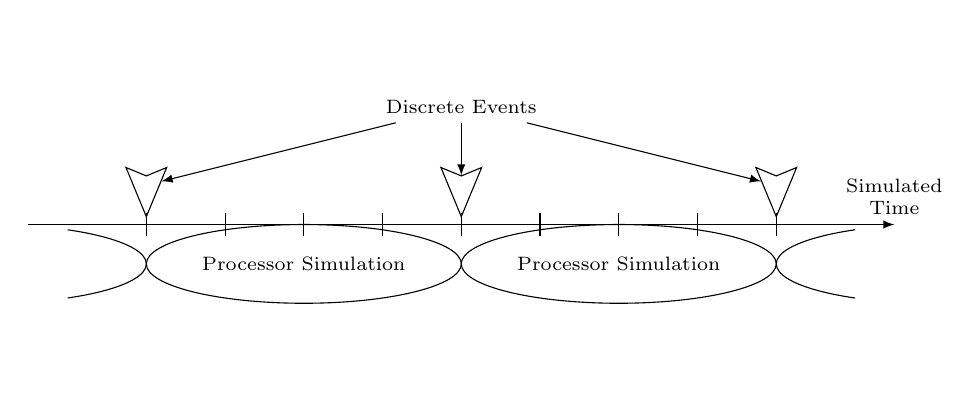
\begin{tikzpicture}[>=latex, font=\scriptsize]
  \draw[->] (-0.5,0) -- (10.5,0) node[pos=1, above, align=center] (sim-time) {Simulated\\Time};

  \begin{scope}
  \clip (0,-2) rectangle (10, 2.5);
  \foreach \x in { 1, 2, 3, 4, 5, 6, 7, 8, 9} {
      \draw (\x,-0.15) -- (\x,0.15) node (tick\x) {};
  };

  \node[shape=dart, draw, shape border rotate=270 ] at (1, 0.5) (event1) {};
  \node[shape=dart, draw, shape border rotate=270 ] at (5, 0.5) (event2) {};
  \node[shape=dart, draw, shape border rotate=270 ] at (9, 0.5) (event3) {};

  \node[above of=event2] (deslabel) {Discrete Events};
  \draw[->] (deslabel) -- (event1);
  \draw[->] (deslabel) -- (event2);
  \draw[->] (deslabel) -- (event3);

  \draw (3,-0.5) ellipse[x radius = 2cm, y radius = 0.5cm] node {Processor Simulation};
  \draw (7,-0.5) ellipse[x radius = 2cm, y radius = 0.5cm] node {Processor Simulation};

  \draw (-1,-0.5) ellipse[x radius = 2cm, y radius = 0.5cm] node {} ;
  \draw (11,-0.5) ellipse[x radius = 2cm, y radius = 0.5cm] node {} ;
  \end{scope}
\end{tikzpicture}
\end{frame}

\begin{frame}{Co-Simulation}
\centering
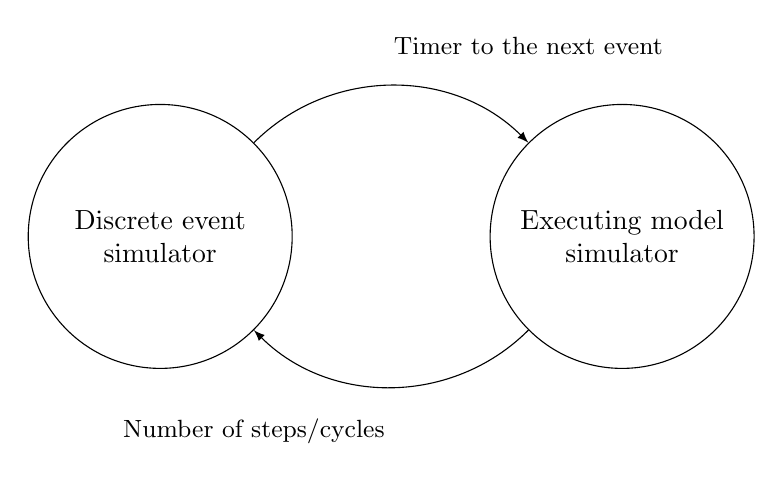
\begin{tikzpicture}[>=latex]
  \node[draw, circle, text width = 3cm, text badly centered] (dessim) {Discrete event simulator};
  \node[draw, circle, text width = 3cm, text badly centered, right = 2.5cm of dessim] (execsim) {Executing model simulator};

  \draw (dessim.45)   edge[bend left = 45, ->] (execsim.135);
  \node[above=1cm of execsim.135] {\small Timer to the next event};
  \draw (execsim.225) edge[->, bend left = 45] (dessim.315);
  \node[below=1cm of dessim.315] {\small Number of steps/cycles};
\end{tikzpicture}
\end{frame}

\section{Multi-Processor Simulation}

\begin{frame}{Simulation of a Multi-Processor System}
\centering
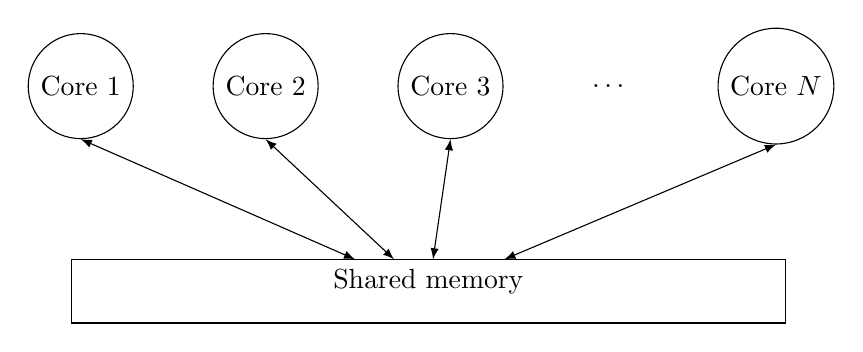
\begin{tikzpicture}[>=latex]
  \node[draw, circle] (core1) {Core 1};
  \node[draw, circle, right = of core1] (core2) {Core 2};
  \node[draw, circle, right = of core2] (core3) {Core 3};
  \node[right = of core3] (dots) {\dots};
  \node[draw, circle, right = of dots] (coren) {Core $N$};

  \coordinate[below = 2.3cm of core1] (c3);
  \coordinate[below = 1.5cm of coren] (c4);

  \node[draw, fit = (c3) (c4), inner ysep=1pt] (shmem) {Shared memory};

  \draw[<->] (core1.south) -- (shmem);
  \draw[<->] (core2.south) -- (shmem);
  \draw[<->] (core3.south) -- (shmem);
  \draw[<->] (coren.south) -- (shmem);
\end{tikzpicture}
\end{frame}

\begin{frame}{Step-by-Step}
\begin{itemize}
\item How to maintain simultaneous instruction simulation for all guest
  processors?\pause~\textit{Execute no more than one instruction at a time.}
\item It will be extremely slow! Maybe it is possible to simulate multiple guest
  instructions without switching?\pause
\item How many?\pause~How much time inter processor communication takes in
  hardware?
\end{itemize}
\end{frame}

% TODO: Add a slide with simulation speed from time quantum dependency using
% qsp-clear-linux.simics

\begin{frame}[fragile]{Temporal Decoupling --- Real Time}
\begin{center}
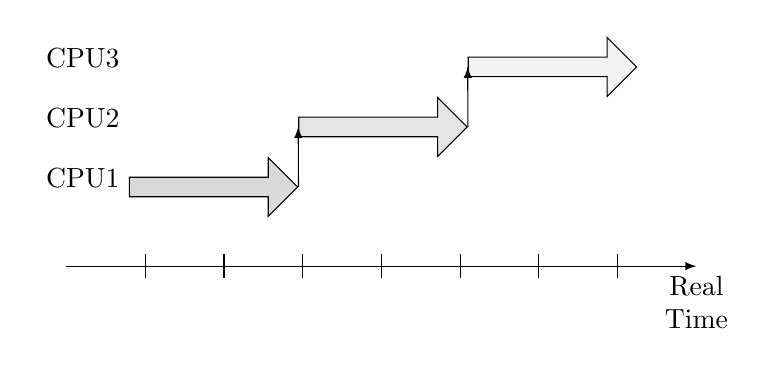
\begin{tikzpicture}[>=latex]
  \draw[->] (0,0) -- (8,0) node[pos=1, below, align=center] (sim-time) {Real\\Time};

  \foreach \x in { 1, 2, 3, 4, 5, 6, 7} {
      \draw (\x,-0.15) -- (\x,0.15) node (tick\x) {};
  };
  \matrix[anchor=south west] at (-0.5,0.5){
    \node {CPU3}; & & & \node[shape=single arrow, draw, text width = 2cm, inner xsep = 0cm, fill=black!5] (arr3) {}; \\
    \node {CPU2}; & & \node[shape=single arrow, draw, text width = 2cm, inner xsep = 0cm, fill=black!10] (arr2) {}; & \\
    \node {CPU1}; & \node[shape=single arrow, draw, text width = 2cm, inner xsep = 0cm, fill=black!15] (arr1) {}; & & \\
  };

  \draw[->] (arr1.east) -- (arr2.west);
  \draw[->] (arr2.east) -- (arr3.west);
\end{tikzpicture}
\end{center}
\end{frame}

\begin{frame}[fragile]{Temporal Decoupling --- Simulated Time}
\begin{center}
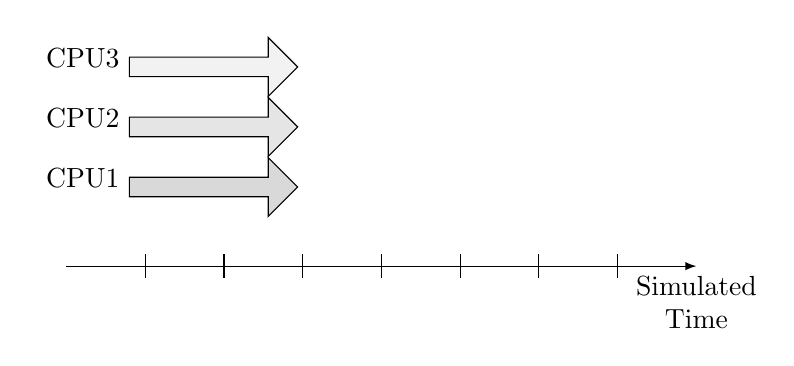
\begin{tikzpicture}[>=latex]
  \draw[->] (0,0) -- (8,0) node[pos=1, below, align=center] (sim-time) {Simulated\\Time};

  \foreach \x in { 1, 2, 3, 4, 5, 6, 7} {
      \draw (\x,-0.15) -- (\x,0.15) node (tick\x) {};
  };
  \matrix[anchor=south west] at (-0.5,0.5){
    \node {CPU3}; & \node[shape=single arrow, draw, text width = 2cm, inner xsep = 0cm, fill=black!5] (arr3) {};  \\
    \node {CPU2}; & \node[shape=single arrow, draw, text width = 2cm, inner xsep = 0cm, fill=black!10] (arr2) {}; \\
    \node {CPU1}; & \node[shape=single arrow, draw, text width = 2cm, inner xsep = 0cm, fill=black!15] (arr1) {}; \\
  };
\end{tikzpicture}
\end{center}
\end{frame}

\begin{frame}{Quantum (Quota)}
Quantum (Quota) --- how many instructions a guest processor can run before
giving control back to the simulator.
\vfill
\begin{itemize}
\item A processor can run fewer instruction than dedicated by the quota.
\item Too big quota can cause unexpected behavior.
\item In a DES-based simulator pseudo-events can be used to cause guest
 processor switch.
\end{itemize}
\end{frame}

\begin{frame}[fragile]{Example \No3: \texttt{qsp-clear-linux.simics}}
Quantum on 8 core system:
\begin{lstlisting}[mathescape=true,keywordstyle=\ttfamily]
simics> cpu-switch-time
Current time quantum: 100.0 $\mu$s
+--------------+------------------------+
|Cycles/quantum|         Clock          |
+--------------+------------------------+
|     200000.00|board.mb.cpu0.core[0][0]|
|     200000.00|board.mb.cpu0.core[0][1]|
|     200000.00|board.mb.cpu0.core[1][0]|
|     200000.00|board.mb.cpu0.core[1][1]|
|     200000.00|board.mb.cpu0.core[2][0]|
|     200000.00|board.mb.cpu0.core[2][1]|
|     200000.00|board.mb.cpu0.core[3][0]|
|     200000.00|board.mb.cpu0.core[3][1]|
+--------------+------------------------+
Default time quantum not set yet
\end{lstlisting}
\end{frame}

\begin{frame}[fragile]{Example \No4: \texttt{qsp-clear-linux.simics}}
Simulated time on 8 core system:
\begin{verbatim}
running> ptime -all
+------------------------+----------+------------+--------+
|       Processor        |  Steps   |   Cycles   |Time (s)|
+------------------------+----------+------------+--------+
|board.mb.cpu0.core[0][0]|1376450747|107696800000|  53.848|
|board.mb.cpu0.core[0][1]| 746604719|107696600220|  53.848|
|board.mb.cpu0.core[1][0]| 746604647|107696600000|  53.848|
|board.mb.cpu0.core[1][1]| 746604686|107696600000|  53.848|
|board.mb.cpu0.core[2][0]| 746604725|107696600000|  53.848|
|board.mb.cpu0.core[2][1]| 746604764|107696600000|  53.848|
|board.mb.cpu0.core[3][0]| 746604803|107696600000|  53.848|
|board.mb.cpu0.core[3][1]| 746604842|107696600000|  53.848|
+------------------------+----------+------------+--------+
\end{verbatim}
\end{frame}

\section*{Conclusions}

\begin{frame}{Conclusions}
\begin{itemize}
\item Simulation with a fixed step.
\item Event-driven simulation.
\item Discrete Event Simulation:
  \begin{itemize}
  \item Event creation.
  \item Event handling.
  \item Event destruction.
  \end{itemize}
\item Co-simulation for executing and non-executing devices.
\item Multi-processor simulation:
  \begin{itemize}
    \item Temporal Decoupling.
    \item Time quantum.
  \end{itemize}
\end{itemize}
\end{frame}

\begin{frame}[allowframebreaks]{Bibliography}
\begin{thebibliography}{99}
  \bibitem{} \textit{John Wiley \& Sons, Inc., ed. by J. Banks}. Handbook of
    Simulation. Principles, Methodology, Advances, Applications, and Practice.
  \bibitem{} \textit{J.~Engblom}. Temporal Decoupling - Are “Fast” and
    “Correct” Mutually Exclusive?
\end{thebibliography}
\end{frame}

\begin{frame}{On the Next Lecture:}
Simulation of architectural state:
\begin{itemize}
\item register file,
\item lazy calculations,
\item large arrays,
\item registers, fields, banks,
\item endianness.
\end{itemize}
\end{frame}

\finalslide

\end{document}
